%%%%%%%%%%%%%%%%%%%%%%%%%%%%%%%%%%%%%%%%%%%%%%%%
%% Intro to LaTeX and Template for Homework Assignments
%% Quantitative Methods in Political Science
%% University of Mannheim
%% Fall 2019
%%%%%%%%%%%%%%%%%%%%%%%%%%%%%%%%%%%%%%%%%%%%%%%%

% created by Marcel Neunhoeffer & Sebastian Sternberg


% This template and tutorial will help you to write up your homework. It will also help you to use Latex for other assignments than this course's homework.

%%%%%%%%%%%%%%%%%%%%%%%%%%%%%%%%%%%%%%%%%%%%%%%%
% Before we get started
%%%%%%%%%%%%%%%%%%%%%%%%%%%%%%%%%%%%%%%%%%%%%%%%

% Make an account on overleaf.com and get started. No need to install anything.

%%%%%%%%%%%%%%%%%%%%%%%%%%%%%%%%%%%%%%%%%%%%%%%%
% Or if you want it the nerdy way...
% INSTALL LATEX: Before we can get started you need to install LaTeX on your computer.
				% Windows: http://miktex.org/download
				% Mac:         http://www.tug.org/mactex/mactex-download.html	
				% There a many more different LaTeX editors out there for both operating systems. I use TeXworks because it looks the same on Windows and Mac.
				

% SAVE THE FILE: The first thing you need to do is to save your LaTeX file in a directory as a .tex file. You will not be able to do anything else unless your file is saved. I suggest to save the .tex file in the same folder with your .R script and where you will save your plots from R to. Let's call this file template_homework1.tex and save it in your Week 1 folder.


% COMPILE THE FILE: After setting up your file, using your LaTeX editor (texmaker, texshop), you can compile your document using PDFLaTeX.
	% Compiling your file tells LaTeX to take the code you have written and create a pdf file
	% After compiling your file, in your directory will appear four new files, including a .pdf file. This is your output document.
	% It is good to compile your file regularly so that you can see how your code is translating into your document.
	
	
% ERRORS: If you get an error message, something is wrong in your code. Fix errors before they pile up!
	% As with error messages in R, google the exact error message if you have a question!
%%%%%%%%%%%%%%%%%%%%%%%%%%%%%%%%%%%%%%%%%%%%%%%%


% Now again for everyone...

% COMMANDS: 
	% To do anything in LaTeX, you must use commands
	% Commands tell LaTeX when to start your document, how you want your document to look, and how to format your document
	% Commands ALWAYS begin with a backslash \

% Everything following the % sign is a comment and will not be used by Latex to compile your document.
% This is very similar to # comments in R.

% Every .tex file usually consists of four parts.
% 1. Document Class
% 2. Packages
% 3. Header
% 4. Your Document

%%%%%%%%%%%%%%%%%%%%%%%%%%%%%%%%%%%%%%%%%%%%%%%%
% 1. Document Class
%%%%%%%%%%%%%%%%%%%%%%%%%%%%%%%%%%%%%%%%%%%%%%%%
 
 % The first command you will always have will declare your document class. This tells LaTeX what type of document you are creating (article, presentation, poster, etc). 
% \documentclass is the command
% in {} you specify the type of document
% in [] you define additional parameters
 
\documentclass[a4paper,12pt]{article} % This defines the style of your paper

% We usually use the article type. The additional parameters are the format of the paper you want to print it on and the standard font size. For us this is a4paper and 12pt.

%%%%%%%%%%%%%%%%%%%%%%%%%%%%%%%%%%%%%%%%%%%%%%%%
% 2. Packages
%%%%%%%%%%%%%%%%%%%%%%%%%%%%%%%%%%%%%%%%%%%%%%%%

% Packages are libraries of commands that LaTeX can call when compiling the document. With the specialized commands you can customize the formatting of your document.
% If the packages we call are not installed yet, TeXworks will ask you to install the necessary packages while compiling.

% First, we usually want to set the margins of our document. For this we use the package geometry. We call the package with the \usepackage command. The package goes in the {}, the parameters again go into the [].
\usepackage[top = 2.5cm, bottom = 2.5cm, left = 2.5cm, right = 2.5cm]{geometry} 

% Unfortunately, LaTeX has a hard time interpreting German Umlaute. The following two lines and packages should help. If it doesn't work for you please let me know.
\usepackage[T1]{fontenc}
\usepackage[utf8]{inputenc}

% The following two packages - multirow and booktabs - are needed to create nice looking tables.
\usepackage{multirow} % Multirow is for tables with multiple rows within one cell.
\usepackage{booktabs} % For even nicer tables.

% As we usually want to include some plots (.pdf files) we need a package for that.
\usepackage{graphicx} 

% The default setting of LaTeX is to indent new paragraphs. This is useful for articles. But not really nice for homework problem sets. The following command sets the indent to 0.
\usepackage{setspace}
\setlength{\parindent}{0in}

% Package to place figures where you want them.
\usepackage{float}

% The fancyhdr package let's us create nice headers.
\usepackage{fancyhdr}

\usepackage[utf8]{vietnam}

\usepackage{tikz}

\usepackage{graphicx}

\usepackage{listings}

\usepackage{amsmath}

\usepackage{hyperref}
\hypersetup{
    colorlinks=true,
    linkcolor=blue,
    filecolor=magenta,      
    urlcolor=cyan,
    pdftitle={Overleaf Example},
    pdfpagemode=FullScreen,
    }

\urlstyle{same}

\usepackage{xcolor}
\usepackage{tcolorbox}

\usepackage{biblatex}
% \addbibresource{refs.bib}

% Import custom code block
\usepackage{graphicx}

% define listing code
\definecolor{codegreen}{rgb}{0,0.6,0}
\definecolor{codegray}{rgb}{0.5,0.5,0.5}
\definecolor{codepurple}{rgb}{0.58,0,0.82}
\definecolor{backcolour}{rgb}{0.95,0.95,0.92}

\lstdefinestyle{code}{
    backgroundcolor=\color{backcolour},   
    commentstyle=\color{codegreen},
    keywordstyle=\color{magenta},
    numberstyle=\tiny\color{codegray},
    stringstyle=\color{codepurple},
    basicstyle=\ttfamily\footnotesize,
    breakatwhitespace=false,         
    breaklines=true,                 
    captionpos=b,                    
    keepspaces=true,                 
    numbers=left,
    firstnumber=1,
    stepnumber=1,                    
    numbersep=5pt,                  
    showspaces=false,                
    showstringspaces=false,
    showtabs=false,                  
    tabsize=2,
    framesep=10pt,
    xleftmargin=10pt,
    xrightmargin=10pt,
    framexleftmargin=16pt,
    framextopmargin=2pt,
    framexbottommargin=2pt, 
    frame=tb, framerule=0pt,
}

\lstdefinestyle{algo}{
    backgroundcolor=\color{backcolour},   
    commentstyle=\color{codegreen},
    keywordstyle=\color{magenta},
    numberstyle=\tiny\color{codegray},
    stringstyle=\color{codepurple},
    basicstyle=\ttfamily\footnotesize\small\linespread{0.8},
    breakatwhitespace=false,         
    breaklines=true,                 
    captionpos=b,                    
    keepspaces=true,                 
    numbers=none,
    firstnumber=1,
    stepnumber=1,                    
    numbersep=5pt,                  
    showspaces=false,                
    showstringspaces=false,
    showtabs=false,                  
    tabsize=2,
    framesep=10pt,
    xleftmargin=10pt,
    xrightmargin=10pt,
    framexleftmargin=16pt,
    framextopmargin=2pt,
    framexbottommargin=2pt, 
    frame=tb, framerule=0pt,
    mathescape=true
}

\lstset{style=code}


%%%%%%%%%%%%%%%%%%%%%%%%%%%%%%%%%%%%%%%%%%%%%%%%
% 3. Header (and Footer)
%%%%%%%%%%%%%%%%%%%%%%%%%%%%%%%%%%%%%%%%%%%%%%%%

% To make our document nice we want a header and number the pages in the footer.

\pagestyle{fancy} % With this command we can customize the header style.

\fancyhf{} % This makes sure we do not have other information in our header or footer.

\lhead{\footnotesize 2022: VIS 01}% \lhead puts text in the top left corner. \footnotesize sets our font to a smaller size.

%\rhead works just like \lhead (you can also use \chead)
\rhead{\footnotesize Linh, Thịnh} %<---- Fill in your lastnames.

% Similar commands work for the footer (\lfoot, \cfoot and \rfoot).
% We want to put our page number in the center.
\cfoot{\footnotesize \thepage} 


%%%%%%%%%%%%%%%%%%%%%%%%%%%%%%%%%%%%%%%%%%%%%%%%
% 4. Your document
%%%%%%%%%%%%%%%%%%%%%%%%%%%%%%%%%%%%%%%%%%%%%%%%

% Now, you need to tell LaTeX where your document starts. We do this with the \begin{document} command.
% Like brackets every \begin{} command needs a corresponding \end{} command. We come back to this later.

\begin{document}


%%%%%%%%%%%%%%%%%%%%%%%%%%%%%%%%%%%%%%%%%%%%%%%%
%%%%%%%%%%%%%%%%%%%%%%%%%%%%%%%%%%%%%%%%%%%%%%%%

%%%%%%%%%%%%%%%%%%%%%%%%%%%%%%%%%%%%%%%%%%%%%%%%
% Title section of the document
%%%%%%%%%%%%%%%%%%%%%%%%%%%%%%%%%%%%%%%%%%%%%%%%

% For the title section we want to reproduce the title section of the Problem Set and add your names.

\thispagestyle{empty} % This command disables the header on the first page. 

\begin{tabular}{p{15.5cm}} % This is a simple tabular environment to align your text nicely 
{\large \bf Một số vấn đề về đồ họa máy tính} \\
Đại học Khoa học Tự nhiên \\
Khoa Toán - Cơ - Tin học \\ 
Khoa học dữ liệu K4 \\
Tháng 12 năm 2022  \\ 
\hline % \hline produces horizontal lines.
\\
\end{tabular} % Our tabular environment ends here.

\vspace*{0.3cm} % Now we want to add some vertical space in between the line and our title.

\begin{center} % Everything within the center environment is centered.
	{\Large \bf Chương 7 - Kĩ thuật đồ họa \\ cho dữ liệu hướng thời gian} % <---- Don't forget to put in the right number
	\vspace{2mm}
	
        % YOUR NAMES GO HERE
	{\bf Nguyễn Mạnh Linh, Nguyễn Đức Thịnh} % <---- Fill in your names here!
		
\end{center}  

\vspace{0.4cm}

%%%%%%%%%%%%%%%%%%%%%%%%%%%%%%%%%%%%%%%%%%%%%%%%
%%%%%%%%%%%%%%%%%%%%%%%%%%%%%%%%%%%%%%%%%%%%%%%%

% Up until this point you only have to make minor changes for every week (Number of the homework). Your write up essentially starts here.

\textit{Tài liệu này được dịch từ cuốn "Ward, M.O. and Grinstein, G. and Keim, D.,  Interactive Data Visualization: Foundations, Techniques, and Applications, Second Edition, CRC Press, 2015", chương số 7 "Visualization Techniques for Time-Oriented Data".}
\\ \\
Trong chương này chúng tôi giải thích chi tiết các kĩ thuật trực quan hóa cho dữ liệu hướng thời gian. Chúng tôi tổ chức và cấu trúc chương theo cuốn sách này [5]. Do đó, trước tiên chúng tôi nhấn mạnh tầm quan trọng của việc xử lý các yếu tố thời gian qua các ví dụ. Thứ hai, chúng tôi đưa ra các khái niệm cần thiết và các khía cạnh của thời gian và dữ liệu hướng thời gian. Các tập dữ liệu cơ bản đã có trong chương 2. Ở chương này, chúng tôi tập trung vào các đặc điểm của thời gian. Thứ ba, chúng tôi cung cấp một cái nhìn tổng quan về các kĩ thuật trực quan hóa khác nhau. Thứ tư, chúng tôi giải thích ngắn gọn về  \textit{TimeBench}, là mô hình và một thư viện phần mềm phân tích dữ liệu hướng thời gian. Chúng tôi kết luận với đánh giá phân loại theo các kĩ thuật trực quan hóa được trình bày và giới thiệu \textit{TimeViz Browser}, là một kho lưu trữ để hỗ trợ các nhà nghiên cứu và học viên trong việc tìm kiếm các kĩ thuật trực quan hóa tích hợp, tiếp theo là các bài đọc, bài tập và đồ án thực hành.
\section{Giới thiệu}
Bản thân thời gian vốn là dữ liệu một chiều, là trung tâm của việc phát hiện xu hướng, xác định các mẫu lặp lại và mối các mối quan hệ trong dữ liệu. Thời gian và dữ liệu hướng thời gian có những đặc điểm riêng biệt đáng để chúng ta nghiên cứu và xử lý như một kiểu dữ liệu riêng. Do tầm quan trọng của dữ liệu hướng thời gian, cấu trúc của nó đã được nghiên cứu trong nhiều ấn phẩm khoa học. 
\\ \\
Các ví dụ sau minh họa tầm quan trọng của thời gian. Hình (\ref{fig:f7.1}) thể hiện ba biểu diễn trực quan khác nhau của cùng một tập dữ liệu hướng thời gian, chứa số ca mắc cúm hàng ngày xảy ra ở miền bắc nước Đức trong khoảng thời gian ba năm. Dữ liệu thể hiện một mô hình tuần hoàn mạnh. Hình ngoài cùng bên trái sử dụng một biểu đồ đường đơn giản để trực quan hóa dữ liệu. Mặc dù thời gian cao điểm có thể được nhận ra dễ dàng, tuy nhiên khi kiểm tra biểu diễn này, hành vi theo chu kì của dữ liệu chỉ có thể được đoán và thật khó để phân biệt các chu kì mà trên thực tế có tồn tại. Ngược lại, hình ở giữa và hình bên phải biểu diễn một vòng tròn nhấn mạnh các đặc tính tuần hoàn của dữ liệu bằng cách sử dụng trục thời gian hình xoắn ốc. Với hình xoắn ốc bên trái, mô hình tuần hoàn không được phát hiện ra. Điều này là do độ dài chu kì được đặt là 24 ngày, không khớp với sự tuần hoàn của dữ liệu. Biểu diễn xoắn ốc bên phải được cài đặt với chu kì 28 ngày ngay lập tức tiết lộ sự tuần hoàn trong dữ liệu. Sự khác biệt có ý nghĩa thống kê về số trường hợp bệnh cúm được báo cáo lần lượt vào Chủ Nhật và Thứ Hai là khá rõ ràng. Chúng ta cũng sẽ thấy sự tuần hoàn này nếu đặt độ dài chu ki là 7 hoặc 14 ngày hoặc một bội (nhỏ) của 7 ngày.
\begin{figure}[H] % places figure environment here   
    \centering % Centers Graphic
    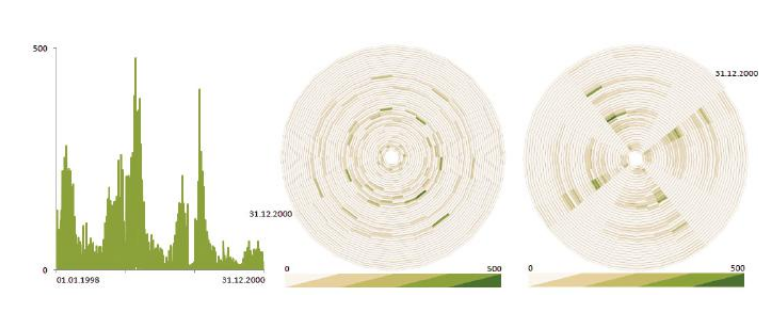
\includegraphics[width=0.8\textwidth]{assets/fg-1.png} 
    \caption{Đặc điểm của thời gian: tuyến tính so với biểu diễn theo chu kỳ của thời gian: những hiểu biết khác nhau
    có thể thu được từ các biểu diễn trực quan tùy thuộc vào việc tuyến tính hay tuần hoàn} % Creates caption underneath graph
    \label{fig:f7.1}
\end{figure}
Ví dụ này đã chứng minh một cách dễ hiểu rằng việc quan sát đặc tính thời gian có thể cải thiện đáng kể ý nghĩa của việc biểu diễn trực quan bằng hình ảnh. Do đó, điều quan trognj là phải chọn một biểu diễn trực quan phù hợp với đặc điểm của dữ liệu (theo chu kì trong trường hợp này) và tham số hóa phù hợp để có thể phát hiện các mẫu lặp lại ẩn trong dữ liệu. 
\\ \\
Trong phần tiếp theo, chúng ta sẽ nghiên cứu các đặc điểm của thời gian và dữ liệu hướng thời gian, thứ cần được xem xét và xử lý để lựa chọn kỹ thuật phù hợp.
\section{Định nghĩa: đặc tính của dữ liệu hướng thời gian}
Phần này bao gồm các khía cạnh chính để mô tả thời gian và dữ liệu hướng thời gian. Điệu quan trọng là phải phân biệt rõ giữa thời gian vật lý và mô hình thời gian trong các hệ thống thông tin. Khi mô hình hóa thời gian trong các hệ thống thông tin, muck tiêu không phải là bắt chước hoàn toàn thời gian vật lý, tuy nhiên để cung cấp mô hình phù hợp nhất để phản ánh các hiện tượng đang được xem xét và hỗ trợ các bài toán phân tích (bằng tay). Hơn nữa, theo Frank [132], không có mô hình đúng duy nhất, có nhiều cách để mô hình hóa thời gian trong các hệ thống thông tin và thời gian cũng được mô hình hóa trong các ứng dụng khác nhau phụ thuộc vào từng bài toán. Các nghiên cứu sâu rộng đã được tiến hành để hình thành khái niệm về thời gian trong nhiều lĩnh vực của khoa học máy tính bảo gồm cả trí tuệ nhân tạo, khai phá dữ liệu, mô phỏng, mô hình, cơ sở dữ liệu ... Chúng tôi phỏng theo các nghiên cứu của Frank [132] và Goralwalla et al [154], trong đó các khía cạnh trực giao chính được trình bày để mô tả các khía cạnh khác nhau của các loại thời gian. Dữ liệu cơ bản được trình bày trong chương 2, chúng tôi tập trung vào các đặc tính của thời gian và dữ liệu hướng thời gian nói riêng. Những khía cạnh này sẽ được mô tả chi tiết sau đây....
\subsection{Các đặc tính của thời gian}
Các đặc tính của thời gian có thể được chia thành các khía cạnh chung yêu cầu mô hình thời gian đầy đủ cũng như tổ chức phân cấp của thời gian và định nghĩa các yêu tố cụ thể. Các khía cạnh tổng quát bao gồm \textit{thang đo}, \textit{phạm vi}, \textit{sắp xếp} và \textit{góc nhìn}.
\begin{itemize}
    \item \textit{Thang đo}: \textit{thứ tự}, \textit{rời rạc}, \textit{liên tục}. Ở góc độ thứ nhất, chúng tôi xem xét thời gian theo thang đo dọc mà các thành phần của mô hình đã được cho trước. Trong miền thời gian theo \textit{thứ tự}, chỉ có quan hệ thứ tự tương đối được biểu diễn (ví dụ như: trước, sau, trong). Trong miền \textit{rời rạc}, khoảng thời gian cũng được xem xét. Các giá trị thời gian có thể được ánh xạ tới một tập các số nguyên, cho phép lập mô hình định lượng các giá trị thời gian. Miền thời gian rời rạc dựa trên đơn vị (ví dụ: giây, phút). Mô hình thời gian \textit{liên tục} đặc trưng bởi ánh xạ đến các số thực. Nghĩa là giữa hai mốc thời gian, tồn tại một mốc thời gian khác (cũng có thể hiểu là mô hình mật độ thời gian).
    \item \textit{Phạm vi}: dựa trên \textit{thời điểm}, dựa trên \textit{khoảng}. Chúng tôi xem xét phạm vi của các yếu tố cơ bản cấu thành nên miền thời gian. Thời gian dựa trên \textit{thời điểm} có thể được biểu diễn như các điểm Euclide rời rạc trong không gian, tức là có mốc thời gian bằng 0. Như vậy không có thông tin được đưa về khoảng giữa 2 thời điểm. Trái ngược với đó, miền dựa theo \textit{khoảng} có độ lớn lớn hơn 0. Khái niệm này cũng có liên quan chặt chẽ đến khái niệm về độ chi tiết, sẽ được bàn luận sau. Ví dụ, giá trị thời gian ngày 1/5/2014 có thể liên quan đến một thời điểm riêng lẻ là 2014-05-01 00:00:00 là một điểm theo miền dựa trên \textit{thời điểm} cũng có thể là đoạn [2014-05-01 00:00:00, 2014-05-01 23:59:99] trong miền dựa trên \textit{khoảng}
    \item \textit{Sắp xếp}: \textit{tuyến tính}, \textit{tuần hoàn}. Tương tự với nhận thức tự nhiên, chúng ta coi thời gian là một quá trình \textit{tuyến tính} từ quá khứ đến tương lai, tức là mỗi giá trị thời gian có một giá trị duy nhất ở hiện tại cũng như tương lai. Trong cách sắp xếp \textit{tuần hoàn} thời gian được xem xét theo các giá trị định kì (ví dụ mùa trong năm).
    \item \textit{Góc nhìn}: \textit{thứ tự}, \textit{nhánh}, \textit{đa góc nhìn}. Miền thời gian theo \textit{thứ tự} xem xét sự kiện xảy ra sau sự kiện khác. Chi tiết hơn, chúng ta cũng có thể phân biệt giữa thứ tự toàn phần và thứ tự một phần. Trong miền thứ tự toàn phần, chỉ một sự kiện có thể xảy ra trong một thời điểm. Trái với đó, các sự kiện đồng thời hoặc chồng chéo được cho phép trong miền thứ tự một phần. Một dạng phức tạp hơn của mô hình thời gian được gọi là \textit{nhánh} thời gian. Trong mô hình này, nhiều nhánh của thời gian có thể được mô tả với các kịch bản khác nhau (ví dụ mô hình lập kế hoạch). Trái ngược với thời gian phân nhánh, chỉ có một đường thực sự diễn ra theo thời gian, mô hình \textit{đa góc nhìn} cho phép nhiều phương án xảy ra đồng thời theo thời gian. Ví dụ nhiều nhân chứng mô tả cùng một tình huống, mỗi người có một góc nhìn khác nhau và kể một câu chuyện khác nhau.
\end{itemize}
Phân loại thứ bậc thời gian và các yếu tố thời gian cụ thể được xác định dựa trên độ chi tiết, đơn vị thời gian và tính xác định.
\begin{itemize}
    \item \textit{Độ chi tiết và lịch}: \textit{rỗng}, \textit{đơn} và \textit{nhiều}. Để giải quyết độ phức tạp về thời gian và đưa ra các độ chi tiết khác nhau, chúng ta có thể sử dụng vài giải thích vắn tắt hữu ích. Về cơ bản \textit{độ chi tiết} là một khái niệm trừu tượng về thời gian (do chúng ta tự định nghĩa) để hình dung thời gian một cách dễ dàng hơn trong cuộc sống (chẳng hạn như giờ, phút, giây). Tổng quan hơn, độ chi tiết mô tả ánh xạ từ thời gian đến các đơn vị nhỏ hơn hoặc lớn hơn. Nếu độ chi tiết và hệ thống lịch được hỗ trợ bởi mô hình thời gian, chúng tôi mô tả nó như \textit{nhiều} chi tiết. Bên cạnh biến thể phức tạp này, có thể chỉ có một \textit{đơn} chi tiết hoặc là \textit{không} có khái niệm trừu tượng nào trong này được hỗ trợ.
    \item \textit{Nguyên thủy thời gian}: \textit{tức thời}, \textit{khoảng thời gian}, \textit{nhịp}. Những nguyên thủy thời gian này có thể được xem như một lớp trung gian giữa các phần tử dữ liệu và miền thời gian. Về cơ bản, thời gian nguyên thủy có thể được chia thành neo nguyên thủy (tuyệt đối) và không neo (tương đối). \textit{tức thời} và \textit{khoảng thời gian} thuộc nhóm đầu tiên, tức là chúng nằm trên một ví trí cố định trên miền thời gian. Ngược lại, một \textit{nhịp} là một tính chất tương đối, tức là nó không có vị trí tuyệt đối trên miền thời gian. Tức thời là mô hình dành cho các điểm riêng lẻ trên trục thời gian (đôi khi còn gọi là thời điểm, ví dụ 10/5/2014), khoảng thời gian là khoảng giữa hai thời điểm (ví dụ từ 10/5/2014 đến 16/5/2014), nhịp là thời lượng (của khoảng) mà không có mốc cố định (ví dụ 6 ngày).
    \item \textit{Tính xác định}: \textit{xác định}, \textit{không xác định}. Sự không chắc chắn là một khía cạnh quan trọng khác cần được xem xét của dữ liệu hướng thời gian. Nếu không có thông tin đầy đủ hay chính xác về thời gian hoặc nếu thời gian gốc được chuyển đổi từ độ chi tiết này sang độ chi tiết khác thì sự không chắc chắn sẽ xuất hiện và cần được xử lý. Ví dụ cho điều này là sự không chính xác đến từ kiến thức thực tế (ví dụ thời điểm trái đất hình thành), các dữ liệu được lập kế hoạch trong tương lai (ví dụ nhiệm vụ cần khoảng 2 đến 3 tháng để hoàn thành) hoặc là các sự kiện không chắc chắn (ví dụ khoảng 2 đến 3 ngày trước). Lưu ý rằng tính không xác định thời gian cũng như tính tương đối của các tham chiếu đến thời gian chủ yếu là các tiêu chuẩn của các phát biểu hơn là các sự kiện mà chúng biểu thị. Tính không xác định có thể được hiểu bởi các thông số rõ ràng (ví dụ bắt đầu sớm nhất và bắt đầu gần nhất của một khoảng thời gian) hoặc ngầm hiểu trong trường hợp đa độ chi tiết nhỏ. Ví dụ, xem xét một câu khẳng định "Hoạt động A bắt đầu vào ngày 14 tháng 5 năm 2014 và kết thúc vào ngày 17 tháng 5 năm 2014" - khẳng định này có thể được mô hình hóa bằng điểm bắt đầu "14/5/2014" và điểm kết thúc "17/5/2014" cả hai đều có độ chi tiết tính đến ngày. Nếu ta nhìn vào khoảng này với độ chi tiết theo giờ, khoảng có thể bắt đầu và kết thúc vào các điểm giữa 0 AM và 12 PM của một ngày nhất định. Chính vì vậy, \textit{tính xác đinh} của tham số thời gian cho trước cần phần được phân tích. Một thông số được biểu diễn khi có kiến thức đầy đủ về  tất cả các khía cạnh của thời gian.
\end{itemize}
Trong phần tiếp theo, chúng tôi khám phá và xác định dữ liệu hướng thời gian một cách chi tiết hơn.
\subsection{Các đặc tính của dữ liệu hướng thời gian}
Cũng như các tính chất của thời gian, dữ liệu có tác động lớn đến việc thiết kế phương pháp trực quan hóa. Chúng ta cùng lược qua những yếu tố chính của dữ liệu liên quan đến thời gian.
\begin{itemize}
    \item \textit{Quy mô}: \textit{định tính}, \textit{định lượng}. Dữ liệu định lượng được dựa trên một thang đo (rời rạc hoặc liên tục). Dữ liệu định tính mô tả tập hợp các phần tử dữ liệu có thứ thự hoặc không có thứ tự.
    \item \textit{Hệ quy chiếu}: \textit{trừu tượng}, \textit{không gian}. Dữ liệu trừu tượng (ví dụ tài khoản ngân hàng) được thu thập trong bối cảnh phi không gian. Dữ liệu không gian (ví dụ dữ liệu điều tra dân số) chứa thông tin về không gian ví dụ như vị trí địa lý.
    \item \textit{Loại dữ liệu}: \textit{sự kiện}, \textit{trạng thái}. Sự kiện có thể được hiểu là các điểm đánh dấu sự thay đổi trạng thái (ví dụ sự khời hành của đoàn tàu), trong khi đó trạng thái đặc trưng cho các giai đoạn liên tục giữa các sự kiện (ví dụ đoàn tàu đang chạy trên đường sắt).
    \item \textit{Số biến}: \textit{đơn biến}, \textit{đa biến}. Dữ liệu đơn biến chỉ chứa một giá trị dữ liệu tại một thời điểm, trong trường hợp đa biến, dữ liệu tại mỗi thời điểm thể hiện bằng nhiều giá trị dữ liệu.
\end{itemize}
Những phạm trù cơ bản này tạo thành cơ sở cho việc lựa chọn, thiết lập kĩ thuật trực quan hóa phù hợp cho dữ liệu hướng thời gian. 
\subsection{Dữ liệu liên quan và thời gian}
Các khía cạnh liên quan của dữ liệu phụ thuộc vào thời gian đã được kiểm tra rộng rãi trong lĩnh vực cơ sở dữ liệu về thời gian [274,397]. Ở đây, chúng tôi điều chỉnh và phát triển các định nghĩa trong lĩnh vực này. Theo đó, bất kì tập dữ liệu nào cũng có liên quan đến 2 miền thời gian: (1) thời gian bên trong và (2) thời gian bên ngoài. 
\\ \\
\textit{Thời gian bên trong} được coi là chiều thời gian vốn có của mô hình dữ liệu. Thời gian bên trong mô tả thời điểm thông tin tồn tại trong tập dữ liệu là hợp lệ. Ngược lại \textit{thời ian bên ngoài} là thời gian nằm ngoài mô hình dữ liệu. Thời gian bên ngoài là cần thiết để mô tả cách một tập dữ liệu phát triển theo thời gian. Dựa vào số biến thời gian nguyên thủy của thời gian bên trong và thời gian bên ngoài, dữ liệu liên quan đến thời gian có thể được phân loại như sau:
\begin{itemize}
    \item \textit{Dữ liệu tĩnh phi thời gian}. Nếu cả thời gian bên trong lẫn bên ngoài bao gồm một yếu tố thời gian thì dữ liệu hoàn toàn không phụ thuộc vào thời gian. Trong chương này chúng ta sẽ không kiểu dữ liệu đó.
    \item \textit{Dữ liệu thời gian tĩnh}. Nếu thời gian bên trong chứa nhiều hơn một yếu tố thời gian nguyên thủy, trong khi thời gian bên ngoài chỉ chứa một thì dữ liệu có thể được xem là phụ thuộc vào thời gian. Vì các giá trị được lưu trong dữ liệu phụ thuộc vào thời gian bên trong , dữ liệu thời gian tĩnh có thể được hiểu là một cái nhìn lịch sử về cách một số mô hình xem xét các yếu tố khác nhau của thời gian trong. Chuỗi thời gian chung là một ví dụ tiêu biểu về dữ liệu thời gian tĩnh. 
    \item \textit{Dữ liệu động phi thời gian}. Nếu thời gian bên trong chỉ chứa một mà thời gian bên ngoài chứa nhiều yếu tố thời gian nguyên thủy thì dữ liệu phụ thuộc vào thời gian bên ngoài. Để cho dễ hiểu, dữ liệu thay đổi qua thời gian thì chúng được gọi là động. Vì thời gian bên trong không được xem xét nên chỉ có trạng thái hiện tại của dữ liệu là bảo toàn. Cái nhìn quá khứ không được duy trì ở đây nữa. Có vài kĩ thuật trực quan hóa sẵn có tập trung vào dữ liệu động phi thời gian, tuy nhiên do thời gian bên trong và thời gian bên ngoài có thể ánh xạ lẫn nhau, một số kĩ thuật trực quan hóa cho dữ liệu tĩnh cũng có thể áp dụng được.
    \item \textit{Dữ liệu động theo thời gian}. Nếu cả thời gian bên trong và bên ngoài đều có nhiều yếu tố thời gian nguyên thủy, thì dữ liệu được xem xét là phụ thuộc vào thời gian. Nói cách khác, dữ liệu chứa các biến phụ thuộc vào thời gian (bên trong) và trạng thái dữ liệu cũng thay đổi theo thời gian (bên ngoài). Thường thì trong trường hợp này, thời gian bên trong và bên ngoài phụ thuộc lẫn nhau và có thể ánh xạ vào nhau. Sự phân biệt rõ ràng giữa thời gian bên trong và bên ngoài thường không được thực hiện bởi các phương pháp trực quan hóa hiện tại bởi xem xét cả 2 chiều thời gian để trực quan hóa là một thách thức.
\end{itemize}
\section{Trực quan hóa dữ liệu hướng thời gian}
Dữ liệu và thời gian đã được trình bày trong phần trước, tuy nhiên chúng ta cũng phải xem xét các vấn đề về thiết kế ở cấp độ biểu diễn trực quan. Để biểu diễn sự phụ thuộc vào thời gian của dữ liệu, ta cần đưa vào trục thời gian. Sự đa dạng của các kĩ thuật trực quan hóa bao gồm các cách tiếp cận rất khác nhau. Để tóm lược sự đa dạng này, chúng tôi tập trung vào 2 tiêu chí cơ bản:
\begin{itemize}
    \item \textit{Ánh xạ của thời gian}. Có hai lựa chọn cho ánh xạ thời gian: ánh xạ thời gian vào không gian và ánh xạ từ thời gian vào thời gian. Khi nói đến ánh xạ từ thời gian vào không gian, điều đó có nghĩa là thời gian và dữ liệu được thể hiện trong một hình ảnh duy nhất. Biểu diễn này không tự thay đổi theo thời gian, đó là lý do tại sao chúng tôi gọi đó là trực quan hóa dữ liệu hướng thời gian \textit{tĩnh}. Ngược lại biểu diễn \textit{động} sử dụng thời gian vật lý để truyền đạt sự phụ thuộc vào thời gian của dữ liệu, nghĩa là thời gian ánh xạ vào thời gian. Các kết quả này trong biểu diễn tự thay đổi theo thời gian (ví dụ bản trình chiếu hay hiệu ứng hoạt họa). Lưu ý rằng, có hay không sự tương tác để điều hướng thời gian không ảnh hưởng đến việc cách tiếp cận trực quan hóa là tĩnh hay động.
    \item \textit{Kích thước của không gian biểu diễn}. Chúng ta có thể phân biệt giữa biểu diễn 2D và 3D của dữ liệu hướng thời gian. Cách trực quan hóa sử dụng không gian 2D phải đảm bảo nhấn mạnh trục thời gian vì chiều thời gian và dữ liệu thường có chung biểu diễn sẵn có. Trong trường hợp biểu diễn 3D, chiều hiển thị thứ 3 được đưa vào. Thực tế, nhiều kĩ thuật sử dụng nó như một chiều dành riêng cho trục thời gian, tách thời gian ra khỏi các chiều dữ liệu khác một cách rõ ràng.
\end{itemize}
\subsection{Phân loại}
Để thuận lời cho việc phân loại một cách dễ dàng và giữ cho phân loại các kĩ thuật trực quan hóa đơn giản, chúng tôi tập trung vào những khía cạnh cốt lõi của dữ liệu, thời gian và trực quan hóa. Qua nhiều ví dụ trực quan hóa, chúng tôi sẽ minh họa những khả năng ứng dụng của chúng và những tính năng của các kĩ thuật trực quan hóa này.
\begin{itemize}
    \item \textbf{Dữ liệu} 
    \item[] \begin{itemize}
        \item \textit{Khung tham chiếu} - trừu tượng, không gian
        \item \textit{Các biến} - đơn biến, đa biến
    \end{itemize}
    \item \textbf{Thời gian}
    \item[] \begin{itemize}
        \item \textit{Sắp xếp} - tuyến tính, tuần hoàn
        \item \textit{Thời gian nguyên thủy} - thời điểm, khoảng
    \end{itemize}
    \item \textbf{Trực quan hóa}
    \item[] \begin{itemize}
        \item \textit{Ánh xạ} - tĩnh, động
        \item \textit{Số chiều} - 2D, 3D
    \end{itemize}
\end{itemize}
Để thiết lập những kĩ thuật trực quan hóa khác nhau cho dữ liệu hướng thời gian, chúng ta cần trả lời những câu hỏi sau:
\begin{itemize}
    \item \textit{Cái gì} được biểu diễn ? \textit{Thời gian và dữ liệu}
    \item \textit{Tại sao} nó được biểu diễn ? \textit{Tác vụ của người dùng}
    \item Nó được biểu diễn \textit{thế nào} ? \textit{Biểu diễn trực quan}
\end{itemize}
Trong chương này, chúng tôi chủ yếu nói về thời gian, dữ liệu và biểu diễn trực quan, bỏ qua những tác vụ của người dùng để mọi thứ trở nên dễ hiểu nhất có thể. Các kĩ thuật trực quan hóa đòi hỏi phải hiểu rõ những khâu cụ thể được thực hiện trong quá trình khai phá dữ liệu và trực quan hóa. MacEachen [281] đã đề xuất một phương pháp ở cấp độ thấp giả quyết một phần cụ thể trong miền thời gian. Các khâu này được định nghĩa bởi một tập các câu hỏi quan trọng mà người dùng có thể tìm kiếm câu trả lời bằng biểu diễn trực quan hóa, ví dụ như \textit{sự tồn tại của thành phần dữ liệu}: liệu thành phần này có tồn tại trong một thời điểm (khoảng) nào đó, hoặc là \textit{tốc độ thay đổi}: thành phần dữ liệu này thay đổi nhanh như thế nào theo thời gian. 
\\ \\
Trong phần tiếp theo, chúng tôi sẽ đưa ra các ví dụ cho mỗi loại được nêu trên.

\subsection{Dữ liệu: Khung tham chiếu - tóm lược}
KronoMiner [488] là một công cụ thăm dò chuỗi thời gian đa năng cung cấp khả năng điều hướng phong phú và hỗ trợ phân tích (hình (\ref{fig:f7.3})). Biễu diễn của nó dựa trên bố cục tâm phân cấp, cho phép người dùng có thể  quan sát chi tiết bằng cách tập trung vào các mảnh khác nhau. Các mảnh dữ liệu có thể được xoay, kéo, co dãn hoặc thu nhỏ một cách dễ dàng, hỗ trợ nhiều kiểu phân tích dữ liệu thời gian. KronoMiner cũng giới thiệu 2 kỹ thuật phân tích: (1) MagicAnalytics Lens, thể hiện mối tương quan của 2 thành phần dữ liệu xếp chồng lên nhau và (2) chế độ Best Match, trong đó một hình cung được hiển thị thể hiện sự tương tự của hai thành phần dữ liệu theo một phép đo cụ thể. 
\begin{figure}[H] % places figure environment here   
    \centering % Centers Graphic
    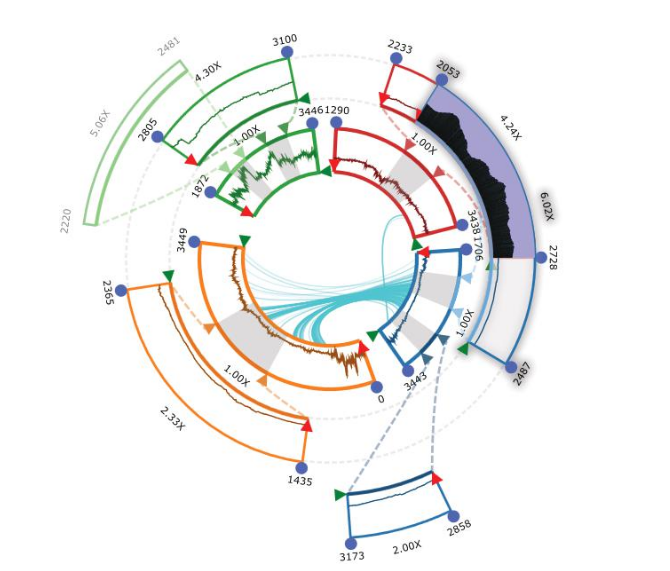
\includegraphics[width=1\textwidth]{assets/fig_7_3.png} 
    \caption{KronoMiner [488]. KronoMiner là một công cụ khám phá chuỗi thời gian đa mục đích cung cấp các tính năng điều hướng và phân tích phong phú} % Creates caption underneath graph
    \label{fig:f7.3}
\end{figure}
\subsection{Dữ liệu: Khung tham chiếu - Không gian}
Tominski và Schulz [415] giới thiệu kĩ thuật trực quan hóa cho dữ liệu thời gian có yếu tố không gian địa lý 2D và thời gian tuyến tính 1D. Ý tưởng là xây dựng một lát cắt không phẳng được gọi là \textit{Great Wall of Space-Time} (hình 7.4) thông qua không-thời gian liên tục 3D (2D+1D). Kiến trúc bức tường này được xây dựng dựa trên các khía cạnh tô tô và hình học của không gian địa lý. Dựa trên một đồ thị lân cận, một đường tô pô được thiết lập tự động hoặc có tương tác. Đường tô pô này được biến đổi thành đường địa lý thông qua những tính chất địa lý của khu vực trên bản đồ. Đường này được dựng thành một bức tường 3D mà chiều thứ 3 có thể được dùng để ánh xạ đến miền thời gian. Những biểu diễn trực quan khác nhau có thể được chiếu lên bức tường này để biểu thị dữ liệu. Bức tường có lợi thế là nó thể hiện một đường khép kín qua không gian mà không có khoảng trống giữa các pixel mang thông tin trên màn hình. 
\begin{figure}[H] % places figure environment here   
    \centering % Centers Graphic
    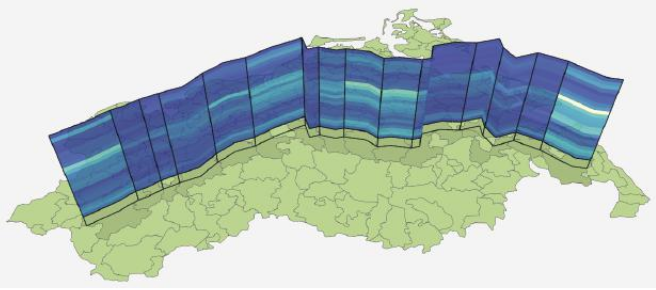
\includegraphics[width=1\textwidth]{assets/fig_7_4.png} 
    \caption{Biểu diễn trực quan hoa của dữ liệu sức khỏe con người sử dụng Great Wall of Space-Time. Một đường trong không gian được thiết lập. Dọc theo đường này, bức tường thể hiện 24 tháng của dữa lioeeuj tại mỗi vùng nó đi qua. Các màu tối thể hiện giá trị dữ liệu thấp, màu sáng thể hiện giá trị cao. Hình trên mô tả số ca mắc cúm } % Creates caption underneath graph
    \label{fig:f7.4}
\end{figure}
\subsection{Dữ liệu: Số biến - Đơn biến}
Trực quan hóa GROOVE (Granularity Overview OVErlay) [262] mở rộng trực quan hóa dựa trên pixel bằng cách phủ lên lớp tổng hợp một hoặc nhiều trong 3 phương pháp: (1) lớp phụ theo màu, (2) lớp phủ theo độ mờ hoặc (3) lớp phủ không gian. Các mức tổng hợp là kết quả của các mức độ chi tiết thời gian khác nhau. Các lớp phủ cho phép đọc vi mô và vĩ mô và trán chuyển động của mắt giữa việc quan sát tổng quan và chi tiết. Với mục đích mình họa, chúng tôi giữ sự hiển thị đơn giản và lượng dữ liệu trực quan không nhiều. Không gian trống xuất hiện do sự bất thường của việc kết hợp các chi tiết tuần và tháng. 
\\ \\
Đầu tiên, các thành phần màu có thể được sử dụng với lớp phủ màu (hình 7.5). Hình này vẽ sơ đồ dữ liệu lưu lượng trong vài tuần. 
\subsection{Dữ liệu: Số biến - Đa biến}
\textit{TimeWheel} [417] là một kỹ thuật để trực quan hóa nhiều biến phụ thuộc thời gian. TimeWheel bao gồm một trục thời gian và nhiều trục cho các biến dữ liệu khác. Trục thời gian được đặt ở trung tâm của hình vẽ để nhấn mạnh đặc tính thời gian của dữ liệu. Các trục của biến dữ liệu khác được ánh xạ bởi các màu khác nhau và dược sắp xếp theo hình tròn quanh trục thời gian. Để trực quan hóa dữ liệu, các đường tỏa ra từ trục thời gian đến mỗi trục khác thiết lập một kết nối giữa thời điểm và các giá trị dữ liệu liên quan. Những đường này tạo thành các nhịp điệu để người dùng xác định mối tương quan với trục thời gian, xu hướng hoặc ngoại lai. Mỗi mẫu như vậy có thể được phân biệt một cách rõ nhất với các trục song song với trục thời gian. Để tập trung vào trục mong muốn, người dùng có thể xoay TimeWheel. Các trục được tập trung có thể được nhấn mạnh bằng cách kéo dài ra. Các trục vuông góc với trục thời gian thì khó giải thích hơn, vì thế  chúng được làm nhạt bớt màu đi và co lại. Khám phá tương tác, bao gồm điều hướng trong thời gian được hỗ trợ thông qua các trục tương tác khác nhau.
\begin{figure}[H] % places figure environment here   
    \centering % Centers Graphic
    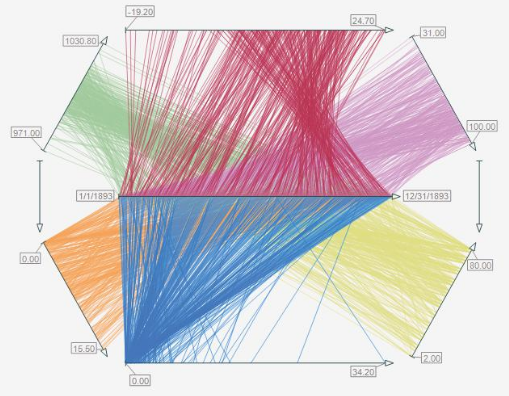
\includegraphics[width=0.8\textwidth]{assets/fig_7_7.png} 
    \caption{Trung tâm của TimeWheel [417] là trục thể hiện thời gian. Các trục khác thể hiện các biến phụ thuộc vào thời gian, hình này thể hiện 8 biến khác nhau tương ứng với 8 trục. Ở giữa, các đường đỏ thể hiện nhiệt độ trung bình, nó tăng khi bắt đầu và giảm về cuối trục thời gian. Các đường xanh dương là lượng mưa. Có một vài ngoại lại với lượng mưa cao nhưng lượng mưa cả năm thì không bất thường (Nguồn: VisAxes) } % Creates caption underneath graph
    \label{fig:f7.7}
\end{figure}
\subsection{Thời gian: Sắp xếp theo trình tự thời gian tuyến tính}
Một trong những cách đơn giản nhất để biểu diễn dữ liệu chuỗi thời gian là sử dụng hệ tọa độ Descartes với trục hoành thể hiện mốc thời gian và trục tung thể hiện giá trị biến định lượng tương ứng. Mỗi cặp gồm mốc thời gian và giá trị tương ứng được thể hiện bằng một điểm trên hệ tọa độ. Cách biểu diễn này thường được gọi là \textit{đồ thị điểm}, \textit{biểu đồ điểm}, hoặc \textit{biểu đồ phân tán} (scatterplot). Harris [170] mô tả cách biểu diễn này là một dạng đồ thị hai chiều trong đó độ lớn của các biến định lượng được thể hiện thông qua khoảng cách của mỗi điểm đến các trục tọa độ. Ngoài dạng cơ bản này còn có nhiều biến thể mở rộng khác, chẳng hạn như kỹ thuật 3D (biểu đồ lớp) hoặc kỹ thuật sử dụng nhiều ký hiệu khác nhau thay vì chỉ đơn thuần là các điểm giống nhau. Kỹ thuật này đặc biệt phù hợp trong trường hợp muốn nhấn mạnh từng giá trị riêng lẻ. Bên cạnh đó, việc biểu diễn dữ liệu bằng các thang đo chung thống nhất sẽ giúp cho người đọc có thể dễ dàng nắm bắt được thông tin một cách trực quan và chính xác nhất. 
\\ \\
Phát triển trên nền tảng của biểu đồ điểm, \textit{biểu đồ đường} cho phép ta thể hiện được mối liên hệ về mặt thời gian giữa các điểm dữ liệu thông qua việc gắn các điểm dữ liệu đó trên một đường nối. Khác với biểu đồ điểm khi tập trung nhấn mạnh vào các điểm dữ liệu riêng lẻ, rời rạc, biều đồ đường sẽ giúp ta tập trung vào xu hướng tổng quan của dữ liệu theo thời gian. Tùy thuộc vào đối tượng đang được xem xét đến ta có thể sử dụng các kiểu kết nối khác nhau giữa các điểm dữ liệu như: đường thẳng, đường bậc thang (liên tục thay đổi giá trị) hoặc đường cong Bezier. Tuy nhiên, dù sử dụng bất kỳ kiểu kết nối nào nêu trên cũng cần lưu ý rằng việc phản ánh giá trị của các điểm nằm giữa hai điểm dữ liệu đã biết đều chỉ mang tính tương đối và ta sẽ không thể đảm bảo chắc chắn về độ chính xác cho mọi điểm dữ liệu được thể hiện trên đường nối. Một vấn đề khác cần lưu ý là việc thiếu dữ liệu. Trong các trường hợp thiếu dữ liệu của một khoảng thời gian nhất định mà người phân tích bỏ qua yếu tố này và chỉ đơn thuần kết nối các điểm dữ liệu liền trước và liền sau khoảng thời gian đó thì nhiều khả năng sẽ dẫn đến những kết luận không chính xác. Do đó, cần có cách thức phù hợp để biểu diễn cho người xem ý thức được vấn đề này, chẳng hạn bằng cách sử dụng các đường nối bằng nét đứt. 
\\ \\ 
Bên cạnh các dạng biểu đồ nêu trên, ta có thể sử dụng một số dạng mở rộng và biến thể khác như: biểu đồ nhiệt, biểu đồ dải, biểu đồ đường lớp, biểu đồ miền, biểu đồ chỉ số hoặc biểu đồ kiểm soát (còn gọi là biểu đồ hành vi – quy trình) (xem [170]).   
\begin{figure}[H] % places figure environment here   
    \centering % Centers Graphic
    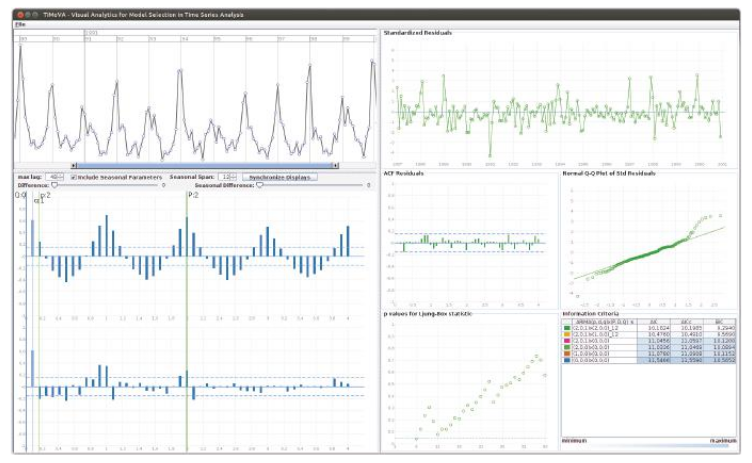
\includegraphics[width=0.8\textwidth]{assets/fig_7_8.png} 
    \caption{iMoVA. Giao diện thể hiện biểu đồ chuỗi thời gian dưới dạng biểu đồ đường (dữ liệu đầu vào; trên cùng bên trái), công cụ lựa chọn mô hình và nhiều chế độ xem khác để định hướng, hỗ trợ quá trình lựa chọn mô hình. (Nguồn: Thực hiện bằng phần mềm nguyên mẫu TiMoVA.)} % Creates caption underneath graph
    \label{fig:f7.8}
\end{figure}
Các loại biểu đồ điểm, biểu đồ đường cũng như các biểu đồ trực quan hóa khác (ví dụ: biểu đồ cột) được sử dụng một cách thường xuyên trong quá trình \textit{TiMoVA (“Ti”: Time series analysis - Phân tích chuỗi thời gian, “Mo”: Model selection - Lựa chọn mô hình, “VA”: applies Visual Analytics methods - áp dụng các phương pháp Phân tích hình ảnh trực quan)} [42]. Phân tích thống kê với dữ liệu chuỗi thời gian là một nhiệm vụ đầy thách thức và đòi hỏi phải được thực hiện bởi các chuyên gia trong nhiều lĩnh vực khác nhau, ví dụ như khi một nhân viên y tế công muốn dự đoán số người cần được điều trị tim mạch trong năm tới. Thông thường, việc lựa chọn mô hình là một nhiệm vụ phức tạp. Chính vì vậy, TiMoVA là một công cụ hữu hiệu, cung cấp giao diện tương tác để định hướng cho người dùng khai phá dữ liệu và lựa chọn mô hình chuỗi thời gian phù hợp. TiMoVA hỗ trợ chuyên gia trong các lĩnh vực ngành nghề trong việc: (1) lựa chọn thứ tự mô hình tương tác thông qua một giao diện trực quan, (2) cung cấp phản hồi về kết quả mô hình trong quá trình chọn thứ tự mô hình một cách trực quan và nhanh chóng tức thì, (3) quyết định về việc có nên cải thiện, thay đổi mô hình hay không (Hình 7.8). Một đánh giá thực nghiệm sử dụng bộ dữ liệu dịch tễ và sự tham gia đánh giá của 02 (hai) chuyên gia thống kê cho thấy TiMoVA hỗ trợ rất hiệu quả trong việc tạo ra một môi trường tương tác khám phá dữ liệu từ đó giúp lựa chọn được các mô hình phù hợp.
\subsection{Thời gian: Sắp xếp theo trình tự thời gian tuần hoàn}
Tominski và Schumann [416] sử dụng mã màu hai tông (two-tone) nâng cao của Saito và cộng sự [354] để trực quan hóa dữ liệu phụ chuỗi thời gian dọc theo hình xoắn ốc. Mỗi đơn vị khoảng thời gian được thể hiện bằng một đoạn duy nhất trên xoắn ốc. Mỗi phân đoạn được chia thành hai phần tô màu theo phương pháp tô màu hai tông. Ưu điểm của việc sử dụng phương pháp tô màu hai tông là nó giúp hiện thực hóa khái niệm tổng quan + chi tiết bằng một thiết kế trực quan. Hai màu được sử dụng trên mỗi đoạn xoắn ốc cho phép người dùng nhanh chóng nhận ra khoảng giá trị của đoạn đó (tổng quan). Nếu ta quan tâm tới một khoảng giá trị nhất định, tỷ lệ của hai màu sẽ giúp biểu thị giá trị dữ liệu cụ thể một cách chính xác (chi tiết). \textit{Xoắn ốc tương tác nâng cao} có thể được điều chỉnh tương tác theo nhiều cách khác nhau. Số lượng đơn vị giai đoạn thời gian, số chu kỳ và các tham số hình học bổ sung sẽ quyết định hình dạng của đường xoắn ốc. Việc biểu diễn dữ liệu chủ yếu được kiểm soát bởi các thang màu sắc đã sử dụng và các tham số như số lượng màu, hướng ánh xạ và chức năng ánh xạ (tuyến tính hay logarit). Việc điều hướng có thể được thực hiện tức thì thông qua việc điều chỉnh trực tiếp xoắn ốc.
\\ \\ 
Nội dung mục này và Hình (\ref{fig:f7.9}) minh họa một hình xoắn ốc nâng cao với mã màu hai tông. Mã giả dưới đây là một ví dụ minh họa cách vẽ một hình xoắn ốc đơn giản trong đó màu sắc và độ rộng của các thanh thể hiện độ lớn giá trị của dữ liệu tương ứng (so sánh hình ảnh ở giữa và bên phải trong Hình (\ref{fig:f7.1})). Các tham số đầu vào bao gồm dữ liệu (\textit{data[]}) - một mảng gồm n giá trị dữ liệu không âm với \textit{max} là giá trị lớn nhất. Tọa độ tâm của hình xoắn ốc được ký hiệu là \textit{cx} và \textit{cy}. Bán kính trong và bán kính ngoài của hình xoắn ốc được cho bởi các tham số \textit{inRad} và \textit{outRad}. Số lượng giá trị dữ liệu hiển thị trong một chu kỳ xoắn ốc đầy đủ, hay nói cách khác là số lượng đoạn thẳng trên mỗi chu kỳ được cho bởi tham số \textit{cyclLen}.
\begin{figure}[H] % places figure environment here   
    \centering % Centers Graphic
    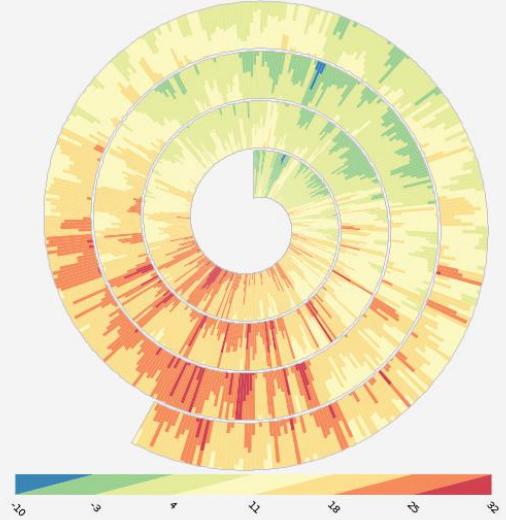
\includegraphics[width=0.8\textwidth]{assets/fig_7_9.png} 
    \caption{Xoắn ốc tương tác nâng cao [416]. Hình xoắn ốc biểu diễn dữ liệu thời tiết trong 3 năm 6 tháng. Mỗi chu kỳ thể hiện 365 giá trị nhiệt độ trung bình hàng ngày ở thành phố Rostock. Ta có thể thấy mùa đông những năm gần đây (chu kỳ ngoài cùng) có khí hậu ôn hòa hơn so với các mùa đông trước. (Nguồn: Hình vẽ được thực hiện bằng công cụ biểu diễn xoắn ốc tương tác nâng cao.)} % Creates caption underneath graph
    \label{fig:f7.9}
\end{figure}
\subsection{Thời gian: Nguyên thủy thời gian – Tức thời}
CareCruiser [163] là một hệ thống trực quan hỗ trợ việc xác định sơ bộ ảnh hưởng của các hoạt động lâm sàng đối với tình trạng của bệnh nhân. Để đạt được mục tiêu này, CareCruiser trực quan hóa các chi tiết trong pháp đồ điều trị kết hợp với các thông số của bệnh nhân, đặc biệt là thông số liên quan đến các quá trình diễn tiến thay đổi theo thời gian. Nó hỗ trợ khai phá thông tin thông qua việc căn chỉnh, đánh dấu màu, lọc và cung cấp thông tin về bối cảnh chung cũng như thông tin chi tiết cần tập trung. Sắp xếp các kế hoạch điều trị lâm sàng theo chiều dọc sẽ giúp đơn giản hóa việc so sánh hiệu quả của các phương pháp điều trị khác nhau hoặc so sánh hiệu quả khác nhau của cùng một phương pháp điều trị nhưng trên nhiều đối tượng bệnh nhân khác nhau. Bên cạnh đó, việc theo dõi hiệu quả của một hoạt động lâm sàng trong tất cả các lần thực hiện (ví dụ: sử dụng lặp lại một loại thuốc nhất định) sẽ giúp tạo điều kiện thuận lợi cho việc so sánh hiệu quả của hoạt động lâm sàng này đối với tình trạng của bệnh nhân. Ba cách phối màu khác nhau được sử dụng để làm nổi bật các phần thú vị trong quá trình phát triển một tham số: việc làm nổi bật (tô đậm) khoảng cách giữa các giá trị thực tế với giá trị dự kiến giúp xác định các giá trị quan trọng; việc làm nổi bật (tô đậm) tiến trình của các giá trị thực tế so với các giá trị ban đầu cho thấy kế hoạch điều trị được áp dụng có tác dụng như đạt mức độ nào so với mong đợi; và việc làm nổi bật độ dốc (sự thay đổi đột ngột) của một giá trị sẽ giúp ta khám phá những tác động tức thời của các hoạt động lâm sàng được áp dụng. Một thanh trượt được cung cấp để lựa chọn màu sắc làm nổi bật cho các sự kiện được chọn (xem Hình 7.10, phía trên cùng) và một cửa sổ cung cấp hình ảnh đã làm mờ thông tin màu bên ngoài đường viền được sử dụng để hỗ trợ quan sát tập trung vào một vùng cần quan tâm cụ thể (ví dụ: phần thời gian nhất định sau khi áp dụng một hành động lâm sàng). Các vùng ít được nhấn mạnh hơn một chút bên ngoài cửa sổ đã nêu trên biểu thị đường cong các giá trị liên tiếp của hoạt động, từ đó cung cấp một số thông tin ngữ cảnh xung quanh cho các giá trị nổi bật mà chúng ta đang quan tâm phân tích. 
\begin{figure}[H] % places figure environment here   
    \centering % Centers Graphic
    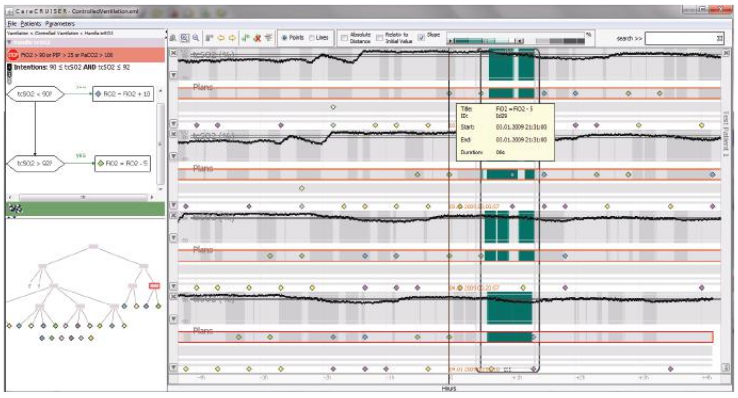
\includegraphics[width=0.8\textwidth]{assets/fig_7_10.png} 
    \caption{CareCruiser [163]. Chế độ xem theo thời gian (ở phía bên phải) sắp xếp các thông số của bệnh nhân cùng với các hoạt động lâm sàng đã được thực hiện (các chấm nhỏ bên dưới biểu đồ đường) dọc theo trục thời gian nằm ngang. Các chế độ xem theo trật tự móc nối logic và trật tự phân cấp ghi lại các kế hoạch điều trị được hiển thị ở phía bên trái. Khu vực đang được chọn ở cửa sổ bên phải thể hiện giá trị tcSO2 của bệnh nhân giảm chậm sau khi áp dụng một hoạt động lâm sàng cụ thể. (Nguồn: Thực hiện bằng phần mềm nguyên mẫu CareCruiser.)} % Creates caption underneath graph
    \label{fig:f7.10}
\end{figure}
\subsection{Thời gian: Nguyên thủy thời gian – Theo khoảng}
Đồng hồ xoắn ốc (SpiraClock) [98] trực quan hóa thời gian bằng cách sử dụng hình ảnh một chiếc đồng hồ. Hình thức thể hiện bao gồm một mặt đồng hồ và hai kim chỉ giờ và chỉ phút. Mặt trong của đồng hồ hiển thị một hình xoắn ốc kéo dài từ viền của đồng hồ về phía tâm của nó. Mỗi chu kỳ của hình xoắn ốc đại diện cho 12 giờ, với thời gian thực được hiển thị ở chu kỳ ngoài cùng và các mốc thời gian tương lai được hiển thị ở gần trung tâm (trong Hình 7.11 là khoảng 9 tiếng sau trong tương lai). Các khoảng thời gian (ví dụ: các cuộc họp) được thể hiện dưới dạng các phân đoạn được tô màu dọc theo hình xoắn ốc. Các phân đoạn này sẽ thể hiện cho ta biết được thời điểm bắt đầu và kết thúc. Từ đó, người dùng cũng có thể nhanh chóng quan sát được xem liệu các cuộc họp nhất định có bị chồng chéo nhau hay chương trình làm việc có quá dày đặc do nhiều sự kiện liên tiếp nhau hay không. Khi thời gian trôi qua, vòng xoắn ốc được cập nhật liên tục và các khoảng thời gian trong tương lai dần dần di chuyển ra ngoài cho đến khi chúng trở thành thời gian hiện tại (thời gian thực). Song song với đó, các khoảng thời gian quá khứ sẽ dần dần mờ đi. Với cách thức hoạt động như trên, SpiraClock là một phiên bản nâng cấp của chiếc đồng hồ cổ điển khi nó cho phép người dùng xem trước các khoảng thời gian của tương lai gần và đồng thời cũng có thể nắm bắt khái quát về các khoảng thời gian quá khứ. SpiraClock cũng cho phép người dùng di chuyển kim đồng hồ để truy cập tới các thời điểm khác nhau, bên cạnh đó ta cũng có thể đánh dấu để làm nổi bật các khoảng thời gian mà chúng ta quan tâm và tạo ra các ghi chú dạng văn bản kèm theo tương ứng.
\begin{figure}[H] % places figure environment here   
    \centering % Centers Graphic
    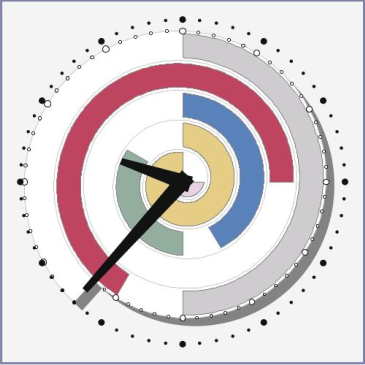
\includegraphics[width=0.8\textwidth]{assets/fig_7_11.png} 
    \caption{SpiraClock [98] được xây dựng dựa trên ý tưởng của màn hình một chiếc đồng hồ. Trong hình, kim phút hiện đang chỉ vào một cuộc họp đang diễn ra. Các cuộc hẹn trong tương lai được xếp dọc theo hình xoắn ốc trên mặt đồng hồ. (Nguồn: Tác giả tổng hợp)} % Creates caption underneath graph
    \label{fig:f7.11}
\end{figure}
\subsection{Trực quan hóa: Ánh xạ tĩnh}
PostHistory [438] khai phá trực quan các mẫu hình (pattern) hoạt động e-mail khác nhau (ví dụ: các mạng xã hội, tốc độ trao đổi e-mail) và vai trò của thời gian trong các mô hình này (xem Hình 7.12). PostHistory lấy người dùng làm trung tâm và tập trung vào các tương tác trực tiếp của một người dùng với những người khác thông qua e-mail. Các mẫu hình được tạo ra từ việc phân tích thông tin tiêu đề e-mail. Vì vậy, không phải nội dung của thư, mà lưu lượng được lưu vết mới là yếu tố được sử dụng làm cơ sở để phân tích các e-mail trao đổi của mọi người theo thời gian. Về cơ bản, giao diện người dùng trực quan hóa hoạt động trao đổi e-mail trong cả một năm và giao diện này được chia thành hai bảng chính: bảng lịch ở bên trái và bảng danh bạ ở bên phải. Bảng lịch hiển thị cường độ hoạt động e-mail hàng ngày trong đó mỗi ô vuông biểu thị một ngày và mỗi hàng biểu thị một tuần. Kích thước của hình vuông được xác định bởi số lượng e-mail nhận được vào ngày đó và màu sắc của nó thể hiện hướng trung bình tính của thư (tức là thư được nhận qua hình thức TO, CC hay BCC). Màu sắc càng sáng thể hiện các thư nhận được trong ngày hôm đó càng được định hướng rõ ràng. Bảng danh bạ được sử dụng để hiển thị tên của những người đã gửi e-mail cho người dùng.
\section{TimeBench: Một mô hình dữ liệu và thư viện hỗ trợ cho việc phân tích trực quan hóa dữ liệu chuỗi thời gian}
Dữ liệu chuỗi thời gian đóng một vai trò quan trọng trong nhiều trường hợp cần phân tích hình ảnh và trực quan hóa, chẳng hạn như khi tìm kiếm những thông tin giá trị từ bộ dữ liệu hồ sơ sức khỏe điện tử hoặc xác định các vấn đề mới phát sinh và các kết nối dễ bị hư hại trong mạng truyền thông. Tuy nhiên, nhiều thư viện phần mềm hỗ trợ phân tích trực quan hiện nay chỉ coi thời gian là một loại dữ liệu số phẳng và vì thế đã giải quyết không triệt để sự phức tạp của miền thời gian, chẳng hạn như độ chi tiết của biểu lịch và các khoảng thời gian. Do đó, các nhà phát triển công cụ, kỹ thuật trực quan hóa nâng cao phải triển khai lặp đi lặp lại các nền tảng liên quan đến thời gian trong bộ mã của họ.
TimeBench [339] là một phần mềm mã nguồn mở và miễn phí cung cấp các cấu trúc dữ liệu nền tảng và thuật toán phục vụ cho việc phân tích và trực quan hóa dữ liệu chuỗi thời gian (http://timebench.org). Khả năng biểu đạt thông tin và khả năng dễ dàng tiếp cận của nó đã được đánh giá thông qua nhiều ứng dụng cụ thể khi giải quyết các thách thức liên quan đến dữ liệu chuỗi thời gian và các nghiên cứu phát triển dài hạn được ở cả cấp độ các chương trình nghiên cứu lẫn các dự án của sinh viên. Hình (\ref{fig:f7.16}) thể hiện 7 ứng dụng khác nhau được phát triển với thư viện TimeBench.
\begin{figure}[H] % places figure environment here   
    \centering % Centers Graphic
    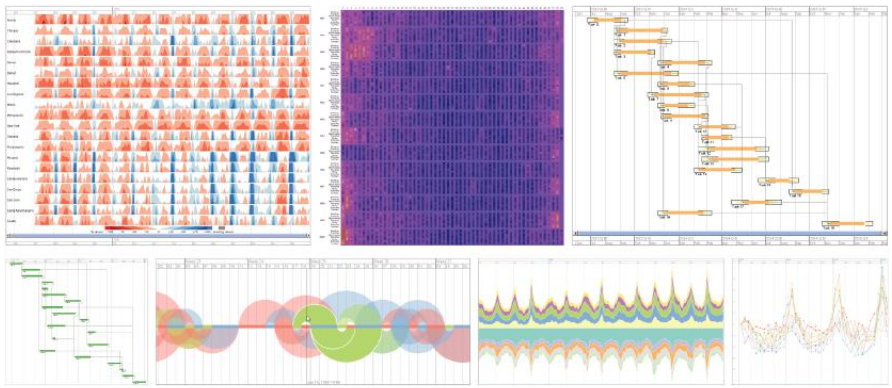
\includegraphics[width=1\textwidth]{assets/fig_7_16.png} 
    \caption{TimeBench [339]. Ví dụ về các ứng dụng được xây dựng dựa trên TimeBench: (1) Dữ liệu sức khỏe hàng tháng của 20 thành phố trong 14 năm trong biểu đồ miền [331]; (2) Dữ liệu sức khỏe hàng ngày trong khoảng thời gian 14 năm được thể hiện trong một biểu đồ GROOVE [262]; (3) Bản kế hoạch dự án sử dụng PlanningLines [4]; (4) Bản kế hoạch dự án dưới dạng biểu đồ Gantt [170]; (5) Sơ đồ vòng cung [451] thể hiện mối quan hệ giữa ba loại sự kiện; (6) Trực quan hóa ThemeRiver [172]; (7) Các biểu đồ đường đi kèm chỉ mục [34]. Dữ liệu sức khỏe từ nghiên cứu NMMAPS [316] được sử dụng trong (1), (2), (5), (6) và (7). (http://timebench.org).} % Creates caption underneath graph
    \label{fig:f7.16}
\end{figure}
\section{Tổng kết}
Trong chương này, chúng ta đã khám phá các khái niệm và phương pháp để trực quan hóa dữ liệu chuỗi thời gian. Chương này cũng đã trình bày cách sử dụng các đặc trưng của dữ liệu chuỗi thời gian trong các kỹ thuật trực quan hóa khác nhau. Các đặc trưng này bao gồm dữ liệu, thời gian và hình ảnh biểu diễn trực quan (xem Phần 3.1). Vì có thể quan sát được những điểm cân xứng và bất cân xứng liên quan đến cách phân loại của chúng tôi, do đó, độc giả nên dành thời gian để xem xét kỹ lưỡng những phần diễn giải cụ thể ở các nội dung đã trình bày.
\begin{itemize}
    \item \textit{Dữ liệu: hệ quy chiếu}. Trong khảo sát này [5], các tác giả chủ yếu tập trung vào loại dữ liệu trừu tượng. Việc biểu diễn dữ liệu chuỗi thời gian trong khung tham chiếu không gian đòi hỏi nhiều hơn đáng kể trong hoạt động thiết kế vì phải đóng gói nhiều thông tin hơn vào trong cùng một biểu đồ trực quan. Đặc biệt là khi đã có các ngành khoa học liên quan đến bản đồ học, vốn là những lĩnh vực nghiên cứu độc lập có lịch sử hình thành và phát triển lâu dài, đã phát triển các phương pháp tiếp cận để kết hợp trực quan hóa các khía cạnh thời gian và không gian của dữ liệu [16, 17, 256]. Hơn nữa, dữ liệu không gian nói chung và không gian địa lý nói riêng cũng đã được trình bày trong Chương 5 và 6.
    \item \textit{Thời gian: sắp xếp}. Hầu hết các kỹ thuật trong khảo sát của chúng tôi [5] tập trung vào việc biểu diễn thời gian theo trình tự tuyến tính; các cách tiếp cận với thời gian theo trình tự tuần hoàn được đề cập ít hơn tương đối. Lý do cho điều này có thể là do người dùng thường quan tâm đến các xu hướng phát triển từ quá khứ, đến hiện tại, đến tương lai hơn là tìm kiếm các chu kỳ tuần hoàn trong dữ liệu.
    \item \textit{Thời gian: nguyên thủy thời gian}. Thời điểm tức thời là nguyên thủy thời gian được sử dụng phổ biến nhất trong khảo sát của chúng tôi [5]. Điều này có vẻ hoàn toàn tự nhiên bởi vì dữ liệu thường được đo lường tại một thời điểm cụ thể. Việc đo lường theo khoảng thời gian thường ít xảy ra hơn và chủ yếu là trong các trường hợp cần đến việc lập kế hoạch.
    \item \textit{Trực quan hóa: ánh xạ}. Rõ ràng, các kỹ thuật ánh xạ tĩnh thì thường phù hợp hơn để biểu diễn trên một trang sách thay vì ánh xạ động. Vì thế, các kỹ thuật trực quan hóa được chọn ở chương này có chút thiên lệch khi tập trung nhiều vào các phương pháp ánh xạ tĩnh. Tuy nhiên, các kỹ thuật ánh xạ động cũng vô cùng quan trọng và nó thường là giải pháp đầu tiên được đưa ra khi trực quan hóa dữ liệu chuỗi thời gian.
    \item \textit{Trực quan hóa: số chiều}. Các phương thức biểu diễn trực quan 2D thường được ưa chuộng hơn so với 3D, vì chúng thường khái quát hơn và do đó dễ hiểu hơn. Và vì thế, một lần nữa các kỹ thuật trực quan hóa đã được giới thiệu trong chương này chủ yếu thiên về phương pháp tiếp cận 2D. Đặc biệt là các kỹ thuật sơ khai có xu hướng gắn liền với không gian hai chiều đơn giản do khả năng tính toán hạn chế khi đó. Tuy nhiên, các công nghệ hiện đại đã giúp các nhà thiết kế trực quan hóa dễ dàng triển khai trực quan hóa 3D hơn và giúp điều hướng góc nhìn của người dùng khi khám phá các không gian thực tế ảo ba chiều. Điều này đặc biệt hữu ích khi trực quan hóa dữ liệu có tham chiếu không gian.
    \item \textit{Trình duyệt TimeViz}. Chúng tôi đã xây dựng một kho lưu trữ (http://survey. timeviz.net) giúp tìm kiếm các phương pháp có sẵn phù hợp với cách thức phân loại đã được giải thích trong Phần \ref{sub:3.1.cate} (xem Hình (\ref{fig:f7.17})). Việc tìm kiếm được thực hiện đơn giản thông qua việc lựa chọn các đặc trưng về thời gian, dữ liệu và biểu diễn trực quan, từ đó các kỹ thuật trực quan hóa phù hợp sẽ được đề xuất dựa trên các đặc trưng đã chọn. Việc cấu trúc kho của chúng tôi trên cơ sở từng trang (per-page) cho phép truy cập dễ dàng khi cần tham khảo nhanh một kỹ thuật cụ thể. Mỗi trang mô tả ngắn gọn bối cảnh, giải thích ý tưởng và các khái niệm chính, đồng thời chỉ ra ứng dụng của một kỹ thuật cụ thể. Phần mô tả chi tiết cũng giới thiệu tham chiếu đến các tài liệu gốc hoặc danh sách các tài liệu tham khảo trong trường hợp có nhiều ấn phẩm cần tham chiếu hoặc nhiều ấn phẩm khác nhau sử dụng cùng một phương pháp. Có thể nói Trình duyệt TimeViz là một công cụ tuyệt vời để tìm kiếm các kỹ thuật trực quan phù hợp theo ba khía cạnh đã nêu trên.
\end{itemize}
\begin{figure}[H] % places figure environment here   
    \centering % Centers Graphic
    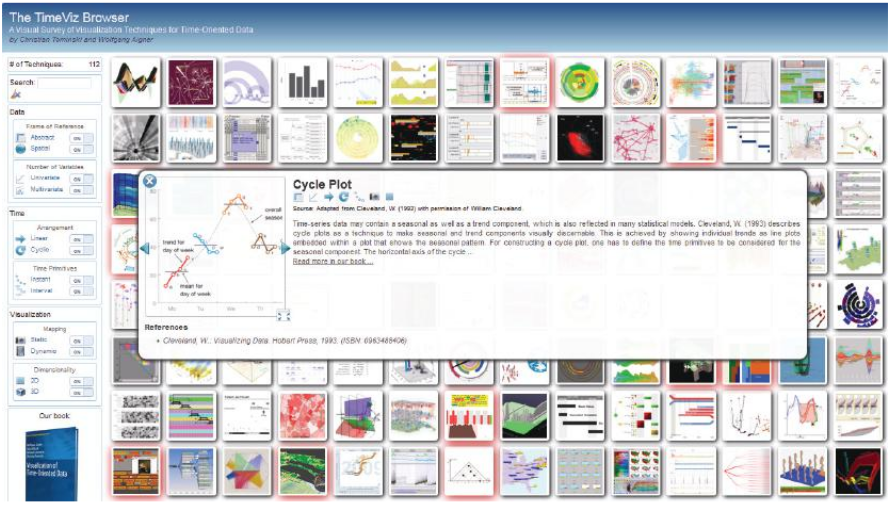
\includegraphics[width=1\textwidth]{assets/fig_7_17.png} 
    \caption{Trình duyệt TimeViz. Kho lưu trữ các kỹ thuật trực quan hóa cho dữ liệu chuỗi thời gian (http://survey.timeviz.net) [5].} % Creates caption underneath graph
    \label{fig:f7.17}
\end{figure}


% \printbibliography

% \begin{thebibliography}{9}
    \text{Ling Liu and Tamer M. Özsu. Encyclopedia of Database Systems. Berlin:
    Springer, 2009.}   
\end{thebibliography}



% \definecolor{mygrey}{rgb}{0.95, 0.95, 0.92}

\section{Bài 2}
Trong phần này chúng ta sẽ xem xét bài toán "Travelling salesman problem" (bài toán 
người giao hàng) - là một trong những bài toán kinh điển và nổi tiếng trong lớp các
bài toán về đồ thị nói chung và bài toán tìm đường đi ngắn nhất nói riêng. \\

\textit{Bài toán: Cho một danh sách các thành phố và khoảng cách từng cặp một, 
tìm đường đi ngắn nhất đi qua mỗi thành phố đúng một lần và quay về điểm xuất phát} \\


Chúng ta có thể mô hình bài toán trên bằng đồ thị như sau: \textit{Cho một đơn đồ thị đầy đủ, 
với các cạnh có trọng số, tìm đường đi xuất phát từ một đỉnh đi qua tất cả các đỉnh 
của đồ thị mỗi đỉnh đúng một lần với tổng trọng số (chi phí) nhỏ nhất.}

Trước hết chúng ta giải bài toán con đơn giản hơn là tìm đường đi với chi phí nhỏ nhất từ
một đỉnh $a$ tới đỉnh $z$ cho trước. Trong bài toán này, không nhất thiết ta phải đi qua 
tất cả các đỉnh của đồ thị. Có nhiều cách tiếp cận bài toán, cách đầu tiên mà ta có thể nghĩ 
ngay tới là \textit{vét cạn (brute force)}, tuy nhiên việc liệt kê toàn bộ cấu hình \
(toàn bộ các đường đi khả dĩ từ $a$ đến $z$) của bài toán rất tốn thời gian. Sau đây ta cùng
xem xét một thuật toán hiệu quả hơn là thuật toán Dijkstra.

\subsection{Thuật toán Dijkstra tìm đường đi ngắn nhất trên đồ thị}
Trước khi giải bài toán tổng quát, ta hãy xem xét một ví dụ đơn giản sau đây:

\begin{figure}[H] % places figure environment here   
    \centering % Centers Graphic
    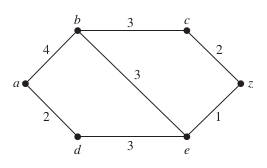
\includegraphics[width=0.4\textwidth]{assets/gr_01.png} 
    \caption{Ví dụ đơn đồ thị với trọng số } % Creates caption underneath graph
    \label{fig:gr_01}
\end{figure}

Tìm đường đi ngắn nhất từ đỉnh $a$ đến đỉnh $z$ trong đồ thị ở hình \ref{fig:gr_01}.\\ 

Trước hết, bắt đầu từ đỉnh $a$, có 2 đỉnh kết nối với $a$ là $b$ và $d$ với trọng số 
lần lượt là $4$ và $2$, đương nhiên $d$ là đỉnh gần $a$ nhất. Chúng ta có thể tìm đỉnh 
gần nhất thứ 2 bằng cách liệt kê tất cả các đường đi với $d$ là đỉnh bắt đầu và đỉnh 
kết thúc không nằm trong tập $\{a, d\}$. Tính từ đỉnh $d$, chỉ có một đường khả dĩ là $e$.
Từ đó ta có tập $\{a, d, e\}$. Tương tự như vậy ta tìm đỉnh tiếp theo với cạnh có trọng số 
nhỏ nhất với $e$ là đỉnh bắt đầu và đỉnh kết thúc không thuộc tập $\{a, d, e\}$, ta được 
đỉnh $z$. Đường đi cuối cùng là $a \to d \to e \to z$. \\

Ví dụ trên thể hiện nguyên lý tổng quát của thuật toán Dijkstra đó là đường đi từ đỉnh $a$
tói đỉnh $z$ có thể được xây dựng bằng cách liệt kê các đường đi và tìm đường có trọng số 
nhỏ nhất để thêm đỉnh đó vào tập đường đi.

Một cách tổng quát ta có thể trình bày thuật toán Dijkstra với lược đồ sau:

\begin{tcolorbox}[colframe=gray,colback=gray!20,left=10pt,right=10pt,top=10pt,bottom=10pt]
    \textbf{Thuật toán Dijkstra} \\
    $G$ là một đơn đồ thị kết nối với trọng số mỗi cạnh dương \\
    $G$ có các đỉnh $a = v_0, v_1, ..., v_n = z$, trọng số 
    $w(v_i, v_j)$ với $w(v_i, v_j) = \infty$ nếu $\{v_i, v_j\}$ không thuộc 
    tập cạnh của $G$

    \begin{itemize}
        \item [] for i = 1 to n 
        \begin{itemize}
            \item [] $L(v_i) = \infty$
        \end{itemize} 
        \item [] $L(a) = 0$
        \item [] $S = \emptyset $ (Khởi tạo các nhãn với nhãn của $a$ là $0$, 
        các nhãn khác bằng $\infty$ và tập $S$ rỗng)
        \item [] while $z \notin S$
        \begin{itemize}
          \item [] $u = a$ đỉnh không thuộc $S$ với $L(u)$ nhỏ nhất
          \item [] $S = S \cup \{u\}$
          \item [] for $v \notin S$
          \begin{itemize}
            \item [] if $L(u) + w(u,v) < L(v)$ then $L(v) = L(u) + w(u,v)$
            (Bước này thêm đỉnh gần nhất vào tập $S$ và cập nhật lại hàm chi phí)
          \end{itemize}
        \end{itemize}
        return $L(z)$ ($L(z)$ là độ dài của đường đi ngắn nhất từ $a$ tới $z$)
    \end{itemize}
  \end{tcolorbox}

\textit{Nhận xét: } Thuật toán Dijkstra đem lại
sự tường minh mà không phải quét qua toàn bộ cấu hình của bài toán, 
ta chỉ cập nhật đỉnh gần với đỉnh cuối cùng nhất, điều đó làm giảm không gian lưu 
trữ so với cách vét cạn (khi ta phải lưu toàn bộ đường đi và chi phí của mọi đường
đi khả dĩ từ đỉnh $a$ tới đỉnh $z$). Độ phức tạp của thuật toán là $O(n^2)$. 
Ta có thể dễ dàng thu được vì ban đầu khi chọn 1 đỉnh, ta cần $(n-1)$ phép so sánh
để tìm được đỉnh gần nhất đầu tiên, tiếp theo ta cần $(n-2)$ phép tính để tìm đỉnh 
gần nhất thứ 2, tiếp tục như vậy cho đến khi thu được đỉnh đích. Số phép tính là tổng 
từ $1$ đến $(n-1)$. \\

Trong thực tế lập trình, chúng ta không nhất thiết phải lưu giá trị cạnh bằng một 
số lớn (vô cùng) mà có thể đánh bằng $0$ và kiểm tra thêm một điều kiện trong vòng 
lặp để tránh sự cồng kềnh của ma trận kề. \\

\href{https://github.com/batman0911/dma_homework/blob/master/hw_02/src/shortest_path.ipynb}{python code} 
    cho bài toán.


\subsection{Bài toán người đưa hàng (TSP)}
Trong mục này chúng ta sẽ xem xét bài toán người đưa hàng đã đề cập ở đầu bài.
Sau khi giải bài toán tìm đường đi ngắn nhất ở mục trước, ta biết rằng bài toán
người đưa hàng không gì khác ngoài việc tìm được đi ngắn nhất khi ta đặt điểm
kết thúc chính là điểm bắt đầu. 
\subsubsection{Thuật toán tìm nghiệm chính xác}
Độ phức tạp thuật toán vét cạn và là $O (n!)$.
Độ phức tạp này tăng rất nhanh theo $n$ . Ví dụ khi bắt đầu từ 1 đỉnh, ta có $(n-1)!$
chu trình Hamilton, tới đỉnh thứ 2 ta còn $(n-2)!$ chu trình Hamilton và tiếp tục như vậy.
Bởi vì ta có thể đi theo thứ tự ngược lại trong chu trình Hamilton nên số chu trình cần
sinh ra để có được lời giải là $(n-1)!/2$. Với số đỉnh bằng $25$, số chu trình được sinh 
ra là $24!/2 \sim 3.1 \times 10^{23}$ - một con số lớn khủng khiếp. Trong thực tế, 
một đơn vị vận chuyển như \textit{Giao hàng tiết kiệm} giao hàng triệu đơn hàng mỗi ngày 
tới các địa điểm khác nhau! Do đó ta gần như không thế tìm được lời giải chính xác của bài 
toán TSP trong thực tế mà cần phải sử dụng các phương pháp xấp xỉ để tìm được một 
đường đi \textit{đủ tốt}.

\subsubsection{Phương pháp xấp xỉ}
Chúng ta sẽ cố gắng đi tìm một cấu hình (chu trình Hamilton) với chi phí không vượt quá
một \textit{ngưỡng} nhất định. Hay nói cách khác $L(H^*_{G}) \leq L(H_{G}) \leq cL(H^*_{G})$,
trong đó $L(H_G)$ là hàm chi phí (tổng các trọng số) của một chu trình Hamilton với
đồ thị $G$ và $H^*_G$ là cấu hình tối ưu của bài toán. Có những thuật toán tìm nghiệm 
xấp xỉ với thời gian đa thức trên đồ thị thỏa mãn bất đẳng thức tam giác với $c = 3/2$. \\

Sử dụng ý tưởng của thuật toán Dijkstra, ta thêm vào tập đỉnh đã đi qua đỉnh lân cận 
gần nhất cho đến khi toàn bộ tập đỉnh đã được đi qua. Độ phức tạp của thuật toán là $O(n^2)$
và ta sẽ cùng xem hệ số $c$ với thuật toán này bằng bao nhiêu. \\

Trước hết, đồ thị $G$ phải thỏa mãn điều kiện bất đẳng thức tam giác 
$w_{ik} + w_{kj} \geq w_{ij}$, với $w_{st}$ là trọng số của cạnh nối đỉnh $s$ và đỉnh $t$.
Điều này cũng khá thực tế khi chi phí bay thẳng từ Hà Nội đến Sài Gòn nên nhỏ hơn là phải 
bay từ Hà Nội vào Đà Nẵng rồi từ Đà Nẵng đi Sài Gòn!

\href{https://github.com/batman0911/dma_homework/blob/master/hw_02/src/travelling_salesman.ipynb}{python code} 
    cho bài toán. \\


% Now we also want to include the graph in our write up.
%  \begin{figure}[H] % places figure environment here   
%     \centering % Centers Graphic
%     \includegraphics[width=0.9\textwidth]{box1.pdf} 
%     \caption{Boxplot of Incumbent Vote share} % Creates caption underneath graph
%   \end{figure}


% Now all we need to answer the question is a neat table. The easiest way to get a nice looking table is to browse to http://www.tablesgenerator.com. Generate your table just like in Word or any other WYSIWYG editor. Then copy and include the code here. I already did that for you.

% \begin{table}[H]
% \centering
% \begin{tabular}{llllllll}
% \multicolumn{1}{c}{\textbf{Variable}} & \multicolumn{1}{c}{\textit{Mean}} & \multicolumn{1}{c}{\textit{Median}} & \textit{Mode} & \textit{Var} & \textit{SD} & \textit{Range} & \textit{IQR} \\ \hline
% Vote                                  & x                                 & x                                   & x             & x            & x           & x              & x            \\
% Growth                                & x                                 & x                                   & x             & x            & x           & x              & x           
% \end{tabular}
% \caption{Measures of central tendency and variability.}
% \label{my-label}
% \end{table}
% You just have to exchange the x for the right value.

\end{document}
